\documentclass{article}
\input{header}

\begin{document}
\rating{2}{4}

A polyomino is called \emph{rectifiable} if there is some number of copies of it that will tile a rectangle.

We say that a polyomino has \emph{rectifiablilty defect} $n$ if we can tile a rectangle missing $n$ holes. (If the polynomial is rectifiable, this metric is $0$.)

\begin{figure}[ht!]
  \[
  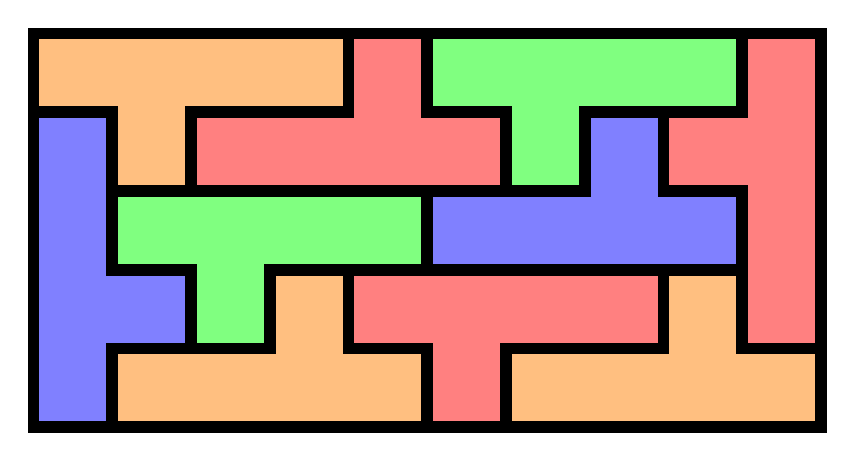
\begin{tikzpicture}
    \draw[fill=blue!50!white, line width=0.15cm, xshift=0cm, yshift=0cm] (0,0)--(1,0)--(1,1)--(2,1)--(2,2)--(1,2)--(1,4)--(0,4)--cycle;
    \draw[fill=orange!50!white, line width=0.15cm,xshift=0cm, yshift=3cm] (0,1)--(1,1)--(1,0)--(2,0)--(2,1)--(4,1)--(4,2)--(0,2)--cycle;
    \draw[fill=green!50!white, line width=0.15cm,xshift=5cm, yshift=3cm] (0,1)--(1,1)--(1,0)--(2,0)--(2,1)--(4,1)--(4,2)--(0,2)--cycle;
    \draw[fill=green!50!white, line width=0.15cm,xshift=1cm, yshift=1cm] (0,1)--(1,1)--(1,0)--(2,0)--(2,1)--(4,1)--(4,2)--(0,2)--cycle;
    \draw[fill=red!50!white, line width=0.15cm,xshift=2cm, yshift=3cm] (0,0)--(4,0)--(4,1)--(3,1)--(3,2)--(2,2)--(2,1)--(0,1)--cycle;

    \draw[fill=red!50!white, line width=0.15cm,xshift=8cm, yshift=1cm] (0,2)--(1,2)--(1,0)--(2,0)--(2,4)--(1,4)--(1,3)--(0,3)--cycle;
    \draw[fill=orange!50!white, line width=0.15cm,xshift=6cm, yshift=0cm] (0,0)--(4,0)--(4,1)--(3,1)--(3,2)--(2,2)--(2,1)--(0,1)--cycle;
    \draw[fill=red!50!white, line width=0.15cm,xshift=4cm, yshift=0cm] (0,1)--(1,1)--(1,0)--(2,0)--(2,1)--(4,1)--(4,2)--(0,2)--cycle;
    \draw[fill=orange!50!white, line width=0.15cm,xshift=1cm, yshift=0cm] (0,0)--(4,0)--(4,1)--(3,1)--(3,2)--(2,2)--(2,1)--(0,1)--cycle;
    \draw[fill=blue!50!white, line width=0.15cm,xshift=5cm, yshift=2cm] (0,0)--(4,0)--(4,1)--(3,1)--(3,2)--(2,2)--(2,1)--(0,1)--cycle;
  \end{tikzpicture}
  \qquad
  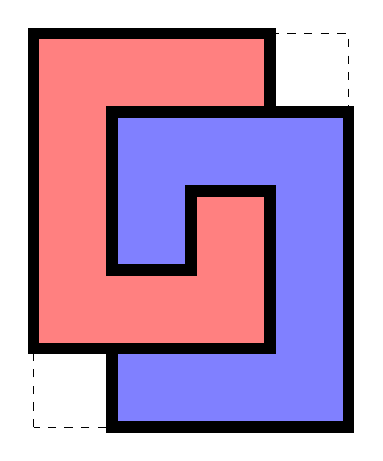
\begin{tikzpicture}
    \draw[dashed] (0,-1) rectangle (4,4);
    \fill[red!50!white, draw=black, line width=0.15cm, xshift=0cm, yshift=0cm] (0,0)--(3,0)--(3,2)--(2,2)--(2,1)--(1,1)--(1,3)--(3,3)--(3,4)--(0,4)--cycle;
    \fill[blue!50!white, draw=black, line width=0.15cm, rotate around={180:(0,0)}, xshift=-4cm, yshift=-3cm] (0,0)--(3,0)--(3,2)--(2,2)--(2,1)--(1,1)--(1,3)--(3,3)--(3,4)--(0,4)--cycle;
  \end{tikzpicture}
  \]
  \caption{
    An example showing a rectifiable $5$-omino, and a non-rectifiable polyomino that has rectifiabilty-defect of $2$.
  }
\end{figure}

\begin{question}
  Let $\operatorname{grd}(n)$ be the greatest rectifiabilty-defect over all $n$-ominoes. What can you say about $\operatorname{grd}(n)$?
\end{question}

\begin{related}
  \item Related question.
  \item If instead, we can have the non-rectifiable polyominoes overlap, what is the least amount of overlap required to tile a rectangle?
  \item What if instead of tiling rectangles, we want to tile squares? Or tile scaled up versions of the polyomino?
\end{related}

\begin{references}
  \item Problem 138.
  \item Peter Kagey, \href{https://peterkagey.com/blog/2025/06/nerd-sniped-by-richard-stanley/}{Nerd sniped by Richard Stanley}
  \item Richard Stanley, \href{https://mathoverflow.net/a/15306/104733}{What are the most attractive Turing undecidable problems in mathematics?}
\end{references}

\end{document}
